\documentclass{article}
\usepackage{graphicx} 
\usepackage{cite}
\usepackage{amsmath,amssymb,amsfonts}
\usepackage{algorithmic}
\usepackage{textcomp}
\usepackage{xcolor}
\usepackage{booktabs}
\usepackage{arydshln}
\usepackage[a4paper, margin=1in]{geometry}
\usepackage{algorithm}
\usepackage{algorithmic}
\usepackage{placeins}
\usepackage{float}
\usepackage{subcaption}

\title{Laboratory 6: Conditional Image Generation}
\author{Víctor Brull Rico \and Guillem Martínez Sambola}
\date{June 8, 2026}

\begin{document}

\maketitle

\section{Introduction}

We present this report on the work carried out in Laboratory~6 on conditional image
generation. Two different approaches are studied.

In the first task, we cover \textit{artistic style transfer} using the CNN-based
algorithm proposed by Gatys \textit{et al.}~\cite{gatys2015neural}. Given a
content image and a style image, the method synthesises a new image that
preserves the semantic structure of the former while adopting the visual
texture and colour palette of the latter. The key insight is that a deep
convolutional network trained for object recognition implicitly separates
content, encoded in high-level feature activations, from style, encoded in
the second-order statistics of those activations across multiple layers.

Moreover, in the second task, we cover \textit{facial animation} using
GANimation~\cite{pumarola2020ganimation}, a GAN-based method that animates a
single RGB portrait by conditioning the generator on Action Unit (AU)
annotations. AUs describe facial muscle movements continuously, allowing fine
control over the intensity and combination of different expressions without
requiring paired training data.

Both tasks are analysed theoretically, with the loss functions identified in
the corresponding code. For the artistic style task, experiments are also
run and the results are evaluated qualitatively.

\section{Methods}
\label{sec:Methods}

\subsection{Artistic Style}

\subsubsection{Overview of the Algorithm}

The neural style-transfer algorithm of Gatys \textit{et al.}~\cite{gatys2015neural}
solves an \emph{image-optimisation} problem: starting from a white-noise image
$\vec{x}$, gradient descent is applied to minimise a composite loss that
simultaneously penalises deviation from the \emph{content} of a reference
photograph $\vec{p}$ and from the \emph{style} of a reference artwork~$\vec{a}$.
The network weights are \textbf{kept fixed throughout}; only the pixel values of
$\vec{x}$ are updated.

\subsubsection{Content Representation and Content Loss}

Each convolutional layer $l$ with $N_l$ filters produces $N_l$ feature maps of
spatial size $M_l$ (height~$\times$~width). The responses are stored in a
matrix $F^l \in \mathbb{R}^{N_l \times M_l}$, where $F^l_{ij}$ is the
activation of filter~$i$ at spatial position~$j$.

Higher layers encode \emph{what} is in the image (objects, their arrangement)
while discarding exact pixel detail; lower layers preserve fine-grained pixel
information. The paper uses layer \texttt{conv4\_2} as the content layer
because it retains high-level structure without sacrificing all spatial detail.

The \textbf{content loss} measures the mean-squared difference between the
feature responses of the generated image~$\vec{x}$ and the content
image~$\vec{p}$ at layer~$l$:

\begin{equation}
    \mathcal{L}_{\text{content}}(\vec{p},\vec{x},l)
    = \frac{1}{2}\sum_{i,j}\!\left(F^l_{ij} - P^l_{ij}\right)^2,
    \label{eq:content_loss}
\end{equation}

\noindent where $P^l$ and $F^l$ are the feature representations of $\vec{p}$
and $\vec{x}$ at layer~$l$, respectively. Minimising this loss drives the
generated image to produce similar activations, thereby preserving the semantic
content.

\subsubsection{Style Representation and Style Loss}

Style is captured not by \emph{where} features activate but by \emph{how they
co-activate} across the spatial extent of a layer. This is formalised through
the \textbf{Gram matrix}:

\begin{equation}
    G^l_{ij} = \sum_{k} F^l_{ik}\, F^l_{jk},
    \label{eq:gram}
\end{equation}

\noindent which contains the inner product between the vectorised feature
maps~$i$ and~$j$ in layer~$l$. The Gram matrix is therefore a
$N_l{\times}N_l$ correlation matrix that captures second-order statistics of
filter responses, discarding spatial arrangement and acting as a texture
descriptor.

\textbf{The style loss} for a single layer compares the Gram matrix of the
generated image~$G^l$ with that of the style image~$A^l$:

\begin{equation}
    E_l = \frac{1}{4N_l^2 M_l^2}
          \sum_{i,j}\!\left(G^l_{ij} - A^l_{ij}\right)^2.
    \label{eq:layer_style_loss}
\end{equation}

The total style loss aggregates contributions from a set of layers $\mathcal{L}$
weighted by $w_l$:

\begin{equation}
    \mathcal{L}_{\text{style}}(\vec{a},\vec{x})
    = \sum_{l \in \mathcal{L}} w_l\, E_l.
    \label{eq:style_loss}
\end{equation}

In practice, layers \texttt{conv1\_1}, \texttt{conv2\_1}, \texttt{conv3\_1},
\texttt{conv4\_1}, and \texttt{conv5\_1} are used with equal weights
$w_l = 1/5$. Including multiple scales allows the style representation to
capture textures at different granularities.

\subsubsection{Total Loss and Optimisation}

The two objectives are combined into a single \textbf{total loss}:

\begin{equation}
    \mathcal{L}_{\text{total}}(\vec{p},\vec{a},\vec{x})
    = \alpha\,\mathcal{L}_{\text{content}}(\vec{p},\vec{x})
    + \beta\,\mathcal{L}_{\text{style}}(\vec{a},\vec{x}),
    \label{eq:total_loss}
\end{equation}

\noindent where $\alpha$ and~$\beta$ are scalar weights that control the
content-style trade-off.  A large ratio $\alpha/\beta$ preserves content at the
expense of style fidelity; a small ratio emphasises stylisation. Typical values
used in~\cite{gatys2015neural} are $\alpha/\beta \in \{10^{-3}, 10^{-4}\}$.

Gradients of $\mathcal{L}_{\text{total}}$ with respect to the pixel values
of~$\vec{x}$ are computed via standard back-propagation and used to update
$\vec{x}$ iteratively (L-BFGS or Adam optimiser). The network weights are
never modified.

\subsubsection{Identification of the Loss in the Code}

The total loss defined in Equation~\eqref{eq:total_loss} is implemented in
\texttt{main.m}. The content loss (Eq.~\ref{eq:content_loss}) appears in the
following lines:

\begin{verbatim}
function loss = contentLoss(transferContentFeatures,contentFeatures,contentWeights)
    loss = 0;
    for i=1:numel(contentFeatures)
        temp = 0.5 .* mean((transferContentFeatures{1,i} - contentFeatures{1,i}).^2,"all");
        loss = loss + (contentWeights(i)*temp);
    end
end
\end{verbatim}

The Gram matrix (Eq.~\ref{eq:gram}) is computed as:

\begin{verbatim}
function gramMatrix = calculateGramMatrix(featureMap)
    [H,W,C] = size(featureMap);
    reshapedFeatures = reshape(featureMap,H*W,C);
    gramMatrix = reshapedFeatures' * reshapedFeatures;
end
\end{verbatim}

The style loss per layer (Eq.~\ref{eq:layer_style_loss}) is:

\begin{verbatim}
function loss = styleLoss(transferStyleFeatures,styleFeatures,styleWeights)
    loss = 0;

    for i=1:numel(styleFeatures)
        tsf = transferStyleFeatures{1,i};
        sf = styleFeatures{1,i};    
        [h,w,c] = size(sf);

        gramStyle = calculateGramMatrix(sf);
        gramTransfer = calculateGramMatrix(tsf);
        sLoss = mean((gramTransfer - gramStyle).^2,"all") / ((h*w*c)^2);
        loss = loss + (styleWeights(i)*sLoss);
    end
end
\end{verbatim}

Finally, the weighted combination (Eq.~\ref{eq:total_loss}) is:

\begin{verbatim}
loss = (params.alpha * cLoss) + (params.beta * sLoss);
\end{verbatim}


\subsection{Facial Animation}

\subsubsection{Overview of GANimation Architecture}

The second task utilizes GANimation~\cite{pumarola2020ganimation} to animate a single facial photograph using continuous muscle activations called Action Units (AUs). The architecture isolates tasks into two primary neural blocks:
\begin{itemize}
    \item \textbf{The Generator ($G$):} Receives the source image and a target vector $\vec{y}$ of desired Action Units. Rather than generating a full scene from scratch, it yields a \textit{Color Content Map ($C$)} and an \textit{Attention Mask ($A$)}. The final composition is blended as:
    \begin{equation}
        \vec{I}_{\text{final}} = A \cdot C + (1 - A) \cdot \vec{I}_{\text{original}}
    \end{equation}
    \item \textbf{The Discriminator ($D$):} Evaluates outputs using two heads: an \textit{Adversarial Critic ($D_{\text{adv}}$)} to verify realistic skin textures, and an \textit{Expression Regressor ($D_{\text{reg}}$)} to estimate Action Unit values and check expression accuracy.
\end{itemize}

\subsubsection{Identification of the Cost Functions in the Code}
Following the implementation code repository, the training routine optimizes a joint objective function. The total costs for the Generator and Discriminator handle four distinct loss terms:

\begin{enumerate}
    \item \textbf{Adversarial Loss (\texttt{criterion_GAN}):} Measures image realism using an LSGAN (Mean Squared Error) or WGAN constraint pattern to verify whether the visual output successfully matches real skin profiles:
\begin{verbatim}
loss_D_g_gan = criterion_GAN(D_g_gan, True)
\end{verbatim}
    \item \textbf{Expression Loss (\texttt{criterion_wreg}):} Evaluates structural regression by computing the mean squared distance between input target Action Units and the muscle activations extracted from the generated face by the critic head:
\begin{verbatim}
loss_G_g_reg = criterion_wreg(D_g_reg, target_aus)
\end{verbatim}
    \item \textbf{Identity / Cycle Consistency Loss (\texttt{criterion_id}):} Guarantees identity tracking by passing the generated facial canvas back to the generator with the subject's original expression vector, penalizing pixel-level structural L1 distances:
\begin{verbatim}
loss_G_back = criterion_id(real_img_back, real_img)
\end{verbatim}
    \item \textbf{Attention Mask Loss:} Enforces an L1 normalization penalty directly on the attention mask array pixels to minimize distortion and keep moving zones tightly localized:
\begin{verbatim}
loss_G_mask = torch.mean(torch.abs(attention_mask))
\end{verbatim}
\end{enumerate}

\subsubsection{Failure Cases and Technical Limitations}
Analyzing the network reveals two distinct scenario limitations:
\begin{itemize}
    \item \textbf{Extreme Head Poses:} When subjects turn completely to the side, features distort because the flat 2D architecture lacks 3D geometric depth knowledge, causing the expression regressor to lose tracking markers.
    \item \textbf{Partial Face Occlusions:} When objects like hands or thick glasses cover skin tissue, the generator treats them as face parts and attempts to warp them into expressions, causing unnatural visual artifacts.
\end{itemize}

\subsubsection{Theoretical Upgrades}
To resolve these errors, two architectural improvements can be proposed from a theoretical standpoint:
\begin{enumerate}
    \item \textbf{3D Morphable Models (3DMM):} Fitting a 3D physical mesh structure over the input face would allow Action Units to deform along a 3D topology, keeping expressions stable across extreme profile angles.
    \item \textbf{Semantic Segmentation Masking:} Incorporating a pre-processing segmentation layer to identify non-face objects (such as hands or glasses) would allow the attention module to lock those pixel zones completely unchanged.
\end{enumerate}


\section{Experiments}
\label{sec:Experiments}

\subsection{Artistic Style}
\label{sec:exp_style}

\subsubsection{Experimental Setup}

All experiments used the VGG-19 network with average-pooling. The content
image was \texttt{lighthouse.png}. Two style images
were selected from the provided data:

\begin{itemize}
\item \textbf{Style~1:} \texttt{starryNight.jpg} - \textit{The Starry Night} by Vincent van Gogh (1889).
\item \textbf{Style~2:} \texttt{dali.jpg} - \textit{The Persistence of Memory} by Salvador Dalí (1931).
\end{itemize}

Experiments were run for \textbf{100 iterations} on CPU. The content layer was \texttt{conv4\_2}
and the style layers were \texttt{conv1\_1} through \texttt{conv5\_1}.
The ratio $\alpha/\beta = 10^{-3}$ was used for both
experiments.

\begin{figure}[H]
\centering
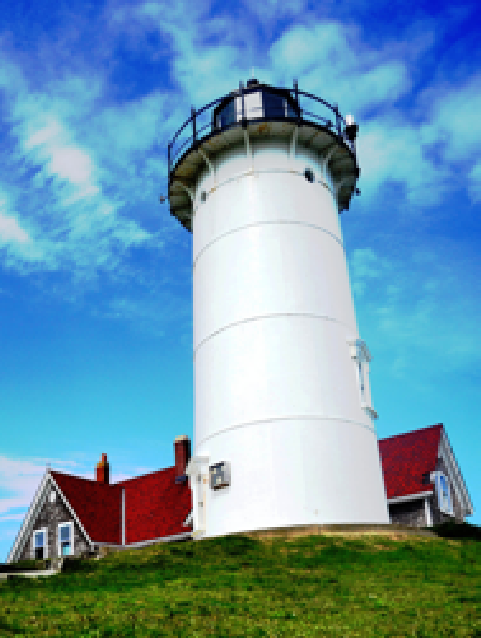
\includegraphics[width=0.3\textwidth]{Figures/lighthouse.png}
\caption{Content image: \texttt{lighthouse.png}.}
\label{fig:content}
\end{figure}

\subsubsection{Results}

% Style 1 Experiment: starryNight.jpg

\begin{figure}[H]
\centering
\begin{subfigure}[b]{0.3\textwidth}
\centering
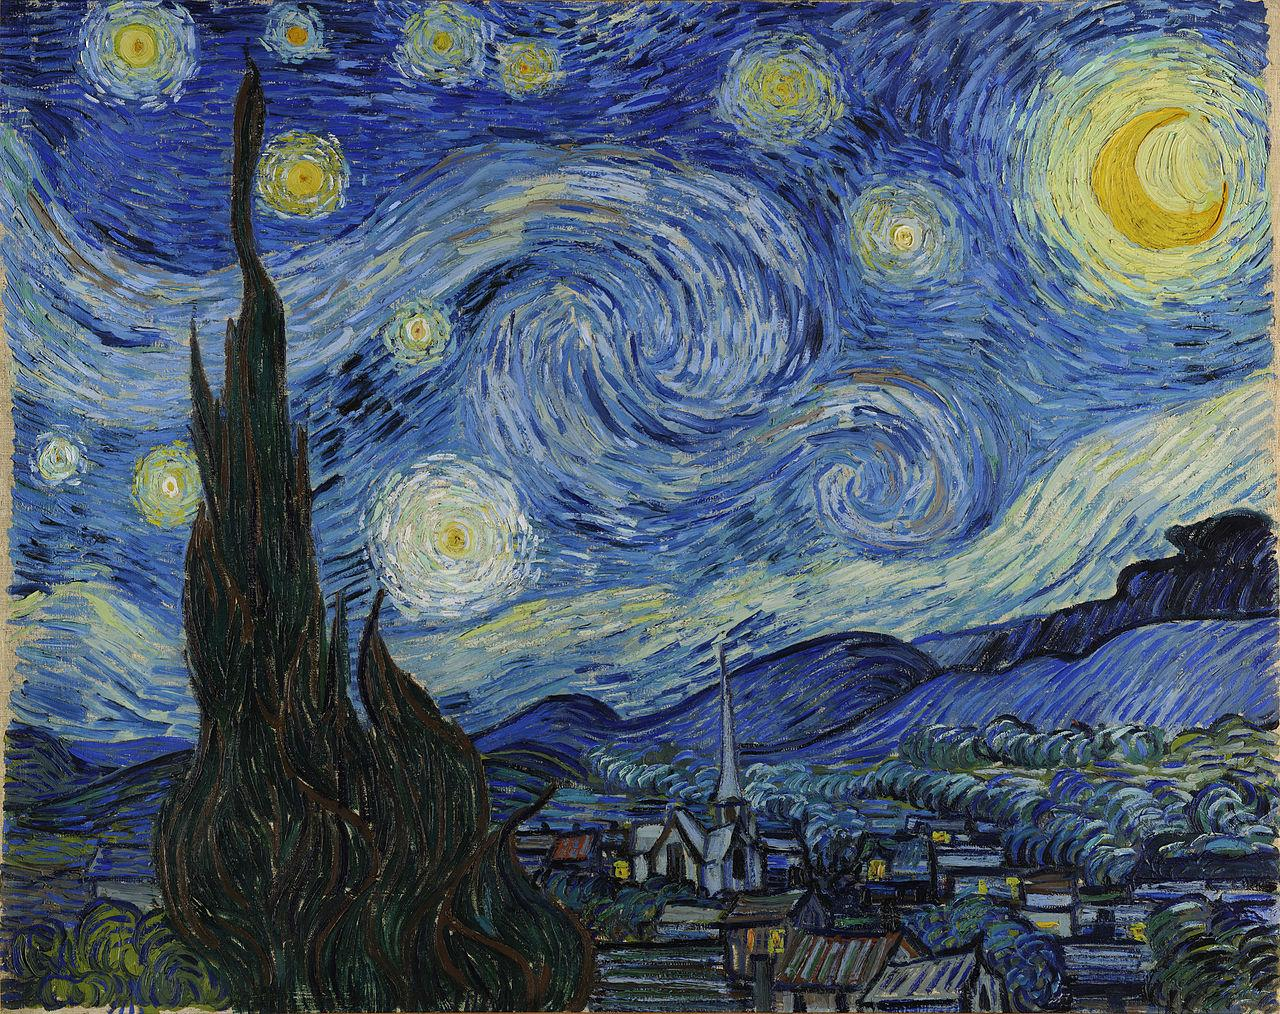
\includegraphics[width=\textwidth]{Figures/starryNight.jpg}
\caption{Style image: \textit{The Starry Night}.}
\label{fig:style1}
\end{subfigure}
\hfill
\begin{subfigure}[b]{0.3\textwidth}
\centering
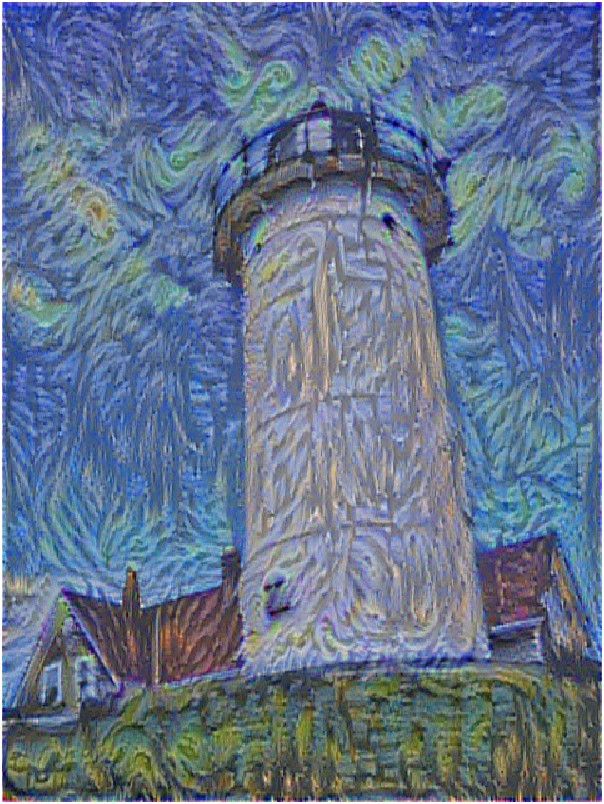
\includegraphics[width=\textwidth]{Figures/output_starryNight.jpg}
\caption{Generated image (100 iter.).}
\label{fig:output1}
\end{subfigure}
\caption{}
\label{fig:experiment1}
\end{figure}

% Style 2 Experiment: dali.jpg

\begin{figure}[H]
\centering
\begin{subfigure}[b]{0.3\textwidth}
\centering
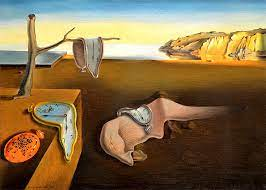
\includegraphics[width=\textwidth]{Figures/dali.jpg}
\caption{Style image: \textit{The Persistence of Memory}.}
\label{fig:style2}
\end{subfigure}
\hfill
\begin{subfigure}[b]{0.3\textwidth}
\centering
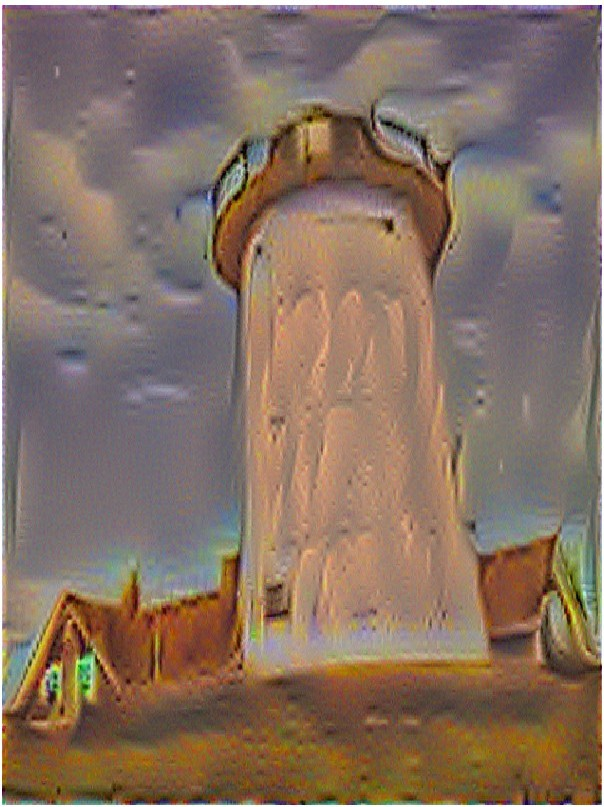
\includegraphics[width=\textwidth]{Figures/output_dali.jpg}
\caption{Generated image (100 iter.).}
\label{fig:output2}
\end{subfigure}
\caption{}
\label{fig:experiment2}
\end{figure}

\subsubsection{Qualitative Evaluation}

\paragraph{Experiment 1: \textit{The Starry Night} style.}
From the generated image, the lighthouse structure is clearly recognisable. For instance, the white tower,
the red-roofed buildings, and the grassy foreground are all preserved. Moreover, the
most visible effect of the style transfer is in the texture and colour palette. The
sky and the surface of the tower have adopted the swirling, wave-like brush
strokes characteristic of van Gogh's painting, and the dominant colours have
shifted towards the blues and yellows of \textit{The Starry Night}. The
semantic content is therefore well maintained, while the artistic texture is
clearly transferred. At 100 iterations the result still shows some roughness,
especially at the edges of the tower. Running for more iterations would likely 
produce a smoother output with stronger stylisation, but the current result already 
demonstrates the algorithm's ability to blend content and style effectively.

\paragraph{Experiment 2: \textit{The Persistence of Memory} style.}
Again, the lighthouse structure is preserved, but the colour
palette has changed significantly. The warm sandy browns and orange tones of
Dalí's painting dominate the output, replacing the original blue sky and green
grass. The textures are less sharp than in Experiment~1, which reflects the
flatter, more blended surface style of Dalí's painting compared to the
thick brush strokes of van Gogh. Some fine details of the lighthouse, such as
the windows, are harder to distinguish in this result, suggesting that the Dalí
style is more aggressive in overwriting low-level detail.

\paragraph{Comparison between the two styles.}
Both experiments confirm that the algorithm successfully separates and
recombines content and style. The van Gogh transfer produces a more visually
striking result because its swirling textures create a strong contrast with the
original photograph. The Dalí transfer is subtler: the content is equally
preserved, but the output looks closer to a colour-graded photograph than to a
painting. This difference is explained by the style images themselves: van
Gogh's work has highly structured, repeated brush-stroke patterns that the Gram
matrices capture easily, while Dalí's painting has smoother gradients and less
repetitive texture.


\section{Conclusion}
\label{sec:Conclusion}

In this laboratory, we have explored two complementary strategies for conditional image
generation based on deep learning.

For the artistic style transfer task, the algorithm of Gatys \textit{et
al.}~\cite{gatys2015neural} was studied and implemented. The method
successfully disentangles content and style by using the feature activations
of a fixed VGG-19 network: content is preserved through layer \texttt{conv4\_2},
while style is captured by Gram matrices computed across five convolutional
layers. The total loss in Equation~\eqref{eq:total_loss} balances both
objectives and is minimised by updating only the pixel values of the generated
image. The experiments showed that both styles were transferred convincingly
at 100 iterations on CPU. The van Gogh style produced a visually striking
result with clear swirling textures and a blue-yellow palette, while the
Dalí style produced a subtler output dominated by warm tones and smooth
gradients. In both cases the content of the lighthouse image remained
recognisable, confirming that the chosen ratio $\alpha/\beta = 10^{-3}$
correctly prioritises content preservation. More iterations or GPU computation
would further improve the quality of the generated images.

For the facial animation task, the GANimation architecture was analysed
theoretically. The generator produces an attention mask and a colour map that
are blended to modify only the relevant facial regions, while the discriminator
jointly ensures visual realism and expression accuracy through adversarial and
regression losses. The main failure cases identified, extreme head poses and
face occlusions, arise from the lack of 3D geometric knowledge in the model.
Two improvements were proposed to address these limitations: incorporating 3D
morphable models to handle out-of-plane rotations, and adding a semantic
segmentation step to prevent non-face regions from being incorrectly warped.

\nocite{*}
\bibliographystyle{ieeetr}
\bibliography{references}

\end{document}